\chapter{RPC \& API \& MOM}
	\section{RPC}
		\subsection{Data Conversion Problems without RPC-Middleware}
			\begin{itemize}
				\item Converting data structures into messages: Data structure as processed by programs must be flattened and reconstructed for exchange (\textbf{(de-)marshalling, (de-)serialization})
				
				\item Converting data types: Sender and receiver may be implemented in different programming
				languages that support different sets of data types or may use different representation for some data types
			\end{itemize}
			$ \Rightarrow $ Solution: Standard data representation; e.g. CORBA: CDR, Web Services: SOAP
			
		\subsection{Other Problems}
			\begin{itemize}
				\item Binding: Finding appropriate services amongst collection of services on
				various machines
				
				\item Fault Handling: Transparent handling of (communication, invocation,\ldots) errors, e.g. Network is down, Machine is busy, Duplicated requests, \ldots
			\end{itemize}
			$ \Rightarrow $ Solution: Interface definition languages (IDLs)
			
		\subsection{IDLs}
			\begin{itemize}
				\item Language to describe services in an abstract manner. Definitions are independent of the PL used to implement clients and services $ \rightarrow $ Supports interoperability btw. languages
				
				\item Code is generated to be invoked by client and code that invokes services on server that deals with all these problems – so-called stubs
			\end{itemize}
			\begin{figure}[h!]
				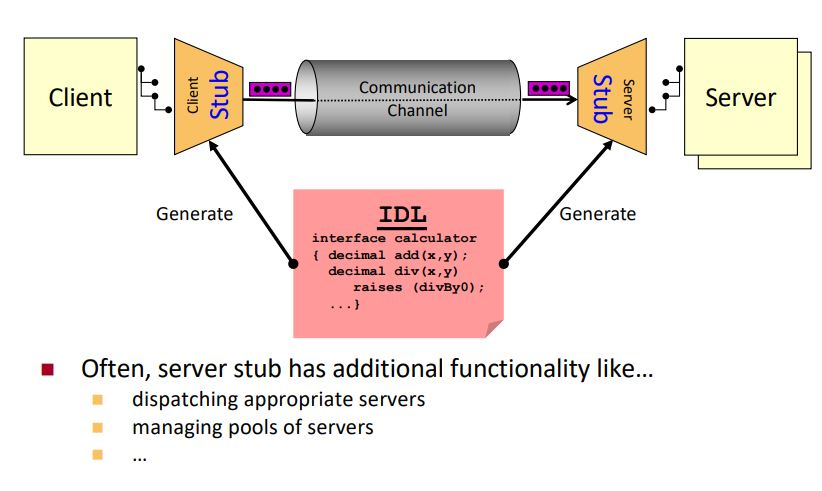
\includegraphics[scale=0.5]{res/idl-stubs.jpg}
			\end{figure}
		
	\section{API}
		API = The set of combined interfaces making the functions of a particular application available in a coherent
		manner.
		\subsection{Structure of a remote API}
			A remote API is split into two parts: The proxy on the client side and the stub on the application side.
			Communication logic is between the proxy and the stub.\\
			client programs against the	proxy and doesn’t know whether the functions used reside on its	local machine or on some remote machine $ \rightarrow $ Local/remote transparency
			
		\subsection{CORBA -- RPC for objects}
			CORBA is an Object Management Group specification for a	\textbf{C}ommon \textbf{ORB} \textbf{A}rchitecture (ORB explained later).\\
			Defines a metamodel for (distributed) objects and a corresponding IDL (CORBA IDL)\\
			Bindings of this IDL to different programming languages are	specified
			
			\subsubsection{Object Request Broker (ORB)}
			\begin{itemize}
				\item mediates remote method invocations in (remote) distributed object systems
				\item supports communication between executables implemented in different programming languages
			\end{itemize}
			\begin{figure}[h!]
				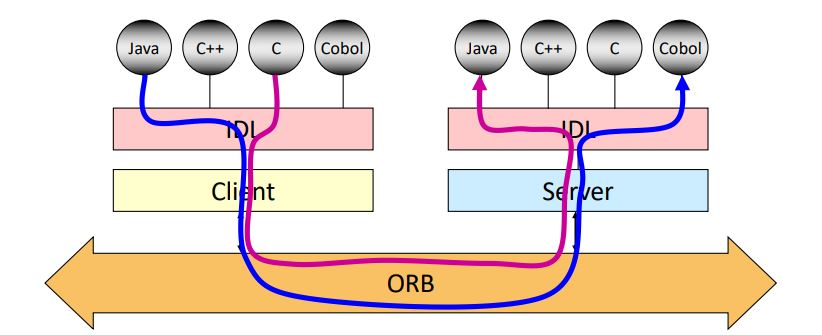
\includegraphics[scale=0.7]{res/orb.jpg}
			\end{figure}
			
			
			\subsubsection{ORB interoperability}
			TODO
			
			
			
			
			
			
			
			
			
			
			
			